% =====================================================================
% Foundations of Physics (FoP) -- Converted Manuscript to Reusable Template
% Omar Iskandarani
% Date: 2025-12-22
% Affiliation: Independent Researcher, Groningen, The Netherlands
% License: © 2025 Omar Iskandarani. All rights reserved. Academic reading/citation only.
% ORCID: 0009-0006-1686-3961
% DOI: 10.5281/zenodo.18018114
%
% Notes:
% - Single .tex file (no \input{...}); figures attached separately.
% - This file is already in the Springer Nature sn-jnl format (FoP-compatible).
% =====================================================================

% =========================
% 1) Document class choice
% =========================
% referee option -> double line spacing for review
% \documentclass[referee,pdflatex,sn-mathphys-num]{sn-jnl}
\documentclass[pdflatex,sn-mathphys-num]{sn-jnl}

% =========================
% 2) Core packages (keep lean)
% =========================
% NOTE: sn-jnl.cls already loads hyperref; to avoid option clashes we
% do not load it again here. Use sn-jnl's built-in hyperlink setup.
\usepackage[T1]{fontenc}
\usepackage[utf8]{inputenc}
\usepackage{lmodern}
\usepackage{microtype}
\usepackage{graphicx}
\usepackage{booktabs}
\usepackage{amsmath,amssymb,amsfonts}
\usepackage{amsthm}
\usepackage{tikz}
\usetikzlibrary{positioning}

% Optional (only if needed)
% \usepackage{bm}
% \usepackage{siunitx}
% \usepackage[title]{appendix}
% \usepackage{xcolor}

% ====================================
% 3) Theorem environments (as needed)
% ====================================
\theoremstyle{thmstyleone}
\newtheorem{theorem}{Theorem}
\newtheorem{proposition}[theorem]{Proposition}

\theoremstyle{thmstyletwo}
\newtheorem{remark}{Remark}

\theoremstyle{thmstylethree}
\newtheorem{definition}{Definition}

% ====================================
% 4) Paper metadata macros (edit here)
% ====================================
\newcommand{\paperdoi}{10.5281/zenodo.18018114}
\newcommand{\papertitle}{Emergent Equivalence Principle from Relational Time and Connection Dynamics}
\newcommand{\papershorttitle}{Emergent Equivalence Principle}
\newcommand{\paperorcid}{0009-0006-1686-3961}
\newcommand{\paperemail}{info@omariskandarani.com}
\newcommand{\papercity}{Groningen}
\newcommand{\papercountry}{The Netherlands}
\newcommand{\paperkeywords}{relational time, equivalence principle, teleparallel gravity, causal structure, quantum clocks}
% Dimensionless deformation parameter
\newcommand{\epsilonL}{\varepsilon_\Lambda} % small energy-to-deformation ratio

% ====================================
% 5) Document starts
% ====================================
\raggedbottom

\begin{document}

    \title[\papershorttitle]{\papertitle}

% ---- Single-author block (FoP style)
    \author*[1]{\fnm{Omar} \sur{Iskandarani}}\email{\paperemail}
    \affil*[1]{\orgname{Independent Researcher}, \orgaddress{\city{\papercity}, \country{\papercountry}}}

% ====================================
% 6) Abstract and keywords
% ====================================
    \abstract{
        The Equivalence Principle (EP) has long anchored the geometric reading of gravitation, yet its foundational status is less clear than the historical narrative suggests. Three lines of work point in the same direction: (i) relativistic kinematics can be fixed on operational grounds from causality alone; (ii) relational formulations of quantum dynamics generate effective time-evolution from clock--system correlations; and (iii) the ``geometric trinity'' shows that curvature-, torsion-, and non-metricity-based formulations are dynamically equivalent while conceptually distinct. I bring these strands together in a conservative framework. Lorentzian causal structure is treated as operationally primary. Mild deformations of a relational Hamiltonian constraint yield gravitational redshift and Newtonian-like interaction terms at low energy. In this setting, the EP reads most naturally as an \emph{emergent} organizing symmetry rather than a primitive axiom. I isolate which parts of the usual EP story are logically prior, which are recovered asymptotically, and where coherence-dependent corrections to redshift should appear. The role of the affine connection is made explicit in mediating inertial and gravitational effects, and the operational regime of validity is expressed through dimensionless parameters directly measurable in quantum-clock interferometry.%
    }
    \keywords{\paperkeywords}

    \maketitle

% ============================================================
    \section{Introduction}\label{sec:intro}
        The Equivalence Principle (EP) is often presented as the conceptual cornerstone of General Relativity (GR), justifying the identification of gravity with spacetime geometry and the universality of free fall \cite{Will2014}. At the same time, several mature ideas now suggest a different ordering of concepts. First, special-relativistic kinematics can be derived from assumptions about observers, signals, and causal order, with no privileged role for electromagnetism \cite{Pineda2026,Zeeman1964}. Second, in relational-time approaches to quantum dynamics, effective redshift and Newtonian-like terms arise from clock--energy couplings in a global constraint, even for otherwise non-interacting subsystems \cite{SinghFriedrich2025,PageWootters1983}. Third, the geometric trinity shows that curvature-, torsion-, and non-metricity-based theories can be dynamically equivalent while remaining conceptually distinct \cite{ManciniTinoCapozziello2025,BeltranJimenez2018,AldrovandiPereira2013}.

        \paragraph{Aim.}
            I give a structural account that respects established phenomenology while reordering the logical dependencies: (i) causality fixes the inertial scaffold; (ii) relational time generates effective gravitational structure at low energy; and (iii) the same empirical content admits inequivalent geometric codings. Read this way, the EP becomes an emergent low-energy symmetry.

        \paragraph{Scope.}
            No new long-range forces are proposed, and no composition-dependent violations are assumed. The goal is to clarify the domain in which the EP is best interpreted as emergent and to identify concrete, coherence-sensitive signatures for quantum-clock experiments.

        \paragraph{Contributions.}
            \begin{enumerate}
                \item An operational summary of how causal order fixes Lorentzian inertial structure (Sec.~\ref{sec:causality}).
                \item A compact operator statement for the low-energy expansion of the relational effective Hamiltonian and its universal energy--energy cross-term (Sec.~\ref{sec:relationaltime}, Prop.~\ref{prop:neumann}).
                \item A perspectival reading that reconciles relational time with connection-based encodings without a globally preferred clock (Sec.~\ref{sec:perspectival}).
                \item A clear account of weak-field redshift and the Newtonian limit in the relational picture, and what is still open about distance dependence (Sec.~\ref{sec:redshift_newton}).
                \item A use of the geometric trinity as geometric underdetermination of shared empirical content (Sec.~\ref{sec:trinity}).
                \item A synthesis in which the EP is an emergent organizing symmetry, with quantum-clock tests singled out as near-term probes (Secs.~\ref{sec:emergence}--\ref{sec:phenom}).
            \end{enumerate}

            \begin{remark}[Didactic recap]
                \emph{In one paragraph.} The paper keeps GR phenomenology intact but reorders the logic: causality fixes the Lorentzian scaffold; relational time with mild constraint deformations generates redshift and a universal energy--energy coupling; and the geometric trinity shows multiple, conceptually distinct encodings with the same dynamics. In that regime, the EP reads as a low-energy symmetry, not a primitive axiom.
            \end{remark}

% ============================================================
    \section{Causality as the Origin of Relativistic Kinematics}\label{sec:causality}

    \subsection{Observers, events, and an operational start}\label{subsec:observers}
        Treat an observer as a localized system carrying a clock and the ability to send/receive signals. Events are indexed by that clock’s reading. This minimal setup captures the idea that spacetime notions are fixed by procedures of registration and communication \cite{Pineda2026}.

    \subsection{Finite signaling and a universal distance}\label{subsec:distance}
        If exchanging information takes finite time, round-trip signal times define distance. Minimizing over admissible messengers picks out a limiting signal class and a maximal transfer speed, with no need to reference a specific field \cite{Pineda2026}.

    \subsection{Causal automorphisms and the Lorentz group}\label{subsec:lorentz}
        Under mild spatial regularity (Euclidean distance in inertial frames), transformations that preserve causal order form the inhomogeneous Lorentz group (up to dilatations) by Alexandrov–Zeeman-type results \cite{Zeeman1964}. Causality thus fixes the Lorentzian kinematic backbone.

        \begin{remark}[Didactic recap]
            \emph{Takeaway.} Start from clocks and signals, not fields. Finite signaling $\Rightarrow$ operational distance; preserving causal order $\Rightarrow$ Lorentz group (modulo scale). This supplies the inertial structure used later by the relational-time construction.
        \end{remark}

% ============================================================
    \section{Relational Time in Quantum Mechanics}\label{sec:relationaltime}

    \subsection{Page--Wootters in brief}\label{subsec:pw}
        Relational-time schemes encode dynamics in correlations between a clock and a system. A stationary global constraint coexists with conditional Schrödinger evolution at fixed clock readings \cite{PageWootters1983,Wootters1984,DeWitt1967}.

    \subsection{A simple deformation and clock--energy coupling}\label{subsec:deformations}
        To model backreaction-like effects, consider
        \begin{equation}
            \hat{J} \equiv \hat{p}_t\otimes \hat{I}_S + \hat{I}_t\otimes \hat{H}_S + \frac{1}{\Lambda}\,\hat{p}_t\otimes \hat{H}_S \approx 0,
            \label{eq:deformed_constraint}
        \end{equation}
        with deformation scale $\Lambda$ \cite{SinghFriedrich2025}. Conditioning on the clock yields an energy-dependent phase rate summarized by
        \begin{equation}
            \hat{H}_{\rm eff} = \hat{H}_S \bigl(\hat{I}_S + \hat{H}_S/\Lambda\bigr)^{-1},
            \label{eq:Heff}
        \end{equation}
        on suitable domains (App.~\ref{app:domains}).

        The parameter $\Lambda$ plays the role of an inverse deformation scale, with $\epsilonL = \lVert \hat{H}_S \rVert / \Lambda \ll 1$ defining the domain of validity for the perturbative expansion. Operationally, $\Lambda^{-1}$ encodes the strength of backreaction between the system and the global clock, analogous to a weak coupling constant in effective theory.

        \begin{proposition}[Low-energy expansion of the relational effective Hamiltonian]
            \label{prop:neumann}
            Let $\hat{H}_S$ be self-adjoint and spectrally supported on a subspace with $\|\hat{H}_S\|<\Lambda$ for some $\Lambda>0$. Then
            \[
                (\hat{I}_S+\hat{H}_S/\Lambda)^{-1}=\sum_{n=0}^{\infty}(-1)^n(\hat{H}_S/\Lambda)^n,
            \]
            so
            \[
                \hat{H}_{\rm eff}=\hat{H}_S-\frac{1}{\Lambda}\hat{H}_S^2+O(\Lambda^{-2}) \qquad (\|\hat{H}_S\|/\Lambda\ll 1).
            \]
            If $\hat{H}_S=\hat{H}_A+\hat{H}_B$ with $[\hat{H}_A,\hat{H}_B]=0$ on that subspace, then the $O(\Lambda^{-1})$ term includes the universal cross-term $-(2/\Lambda)\,\hat{H}_A\otimes \hat{H}_B$.
        \end{proposition}

        \begin{remark}
            The spectral restriction can be read as a low-energy condition or enforced by a bounded-spectrum truncation of the clock/system. That is the regime in which $\Lambda^{-1}$ is a controlled perturbation \cite{SinghFriedrich2025}.
        \end{remark}

    \subsection{Composite systems and emergent interaction}\label{subsec:emergent}
        For $\hat{H}_S=\hat{H}_A+\hat{H}_B$ with $|\hat{H}_S|\ll\Lambda$, expanding \eqref{eq:Heff} gives
        \begin{equation}
            \hat{H}_{\rm eff} \approx \hat{H}_A+\hat{H}_B -\frac{1}{\Lambda}\bigl(\hat{H}_A^2+\hat{H}_B^2+2\,\hat{H}_A\otimes \hat{H}_B\bigr)+O(\Lambda^{-2}),
            \label{eq:Heff_expand}
        \end{equation}
        i.e., a universal energy--energy coupling. With an external identification of distance, this matches the Newtonian form in the weak-field limit (Sec.~\ref{sec:redshift_newton}).

        \begin{remark}[Didactic recap]
            \emph{Plain language.} The clock couples to the system through the constraint. At low energy, that acts like a small correction to the system Hamiltonian: a universal energy–energy term appears between parts $A$ and $B$. This is the seed of both redshift and Newtonian-like behavior later on.
        \end{remark}

% ============================================================
    \section{Perspectival Structure of Relational Time and Gravity}\label{sec:perspectival}
    A durable lesson from quantum foundations is that physically meaningful descriptions are local to a context. In an endo-theoretic perspectival view, perspectives come with finite resolution and context-dependent Boolean algebras; a single global Boolean valuation is unavailable \cite{KarakostasZafiris2025}. Page--Wootters-type constructions fit this picture: each clock choice defines a local temporal ordering while the global state remains stationary \cite{PageWootters1983,Wootters1984}.

    When gravitational effects are modeled by universal clock--energy couplings, proper time is best treated as an observable in correlations. Gravitational time dilation then records a mismatch between clock perspectives rather than the action of a background metric \cite{SinghFriedrich2025}. The geometric trinity is compatible with this: distinct geometric codings (curvature, torsion, non-metricity) summarize the same local dynamical content \cite{BeltranJimenez2018,AldrovandiPereira2013,ManciniTinoCapozziello2025}. In that light, the EP reads as a low-energy compatibility condition among local perspectives.

    \begin{remark}[Didactic recap]
        \emph{Intuition.} No single, globally preferred clock; each clock defines a valid local time. Geometry (curvature/torsion/non-metricity) is then a way to \emph{summarize} how these local descriptions fit together, not a unique underlying picture.
    \end{remark}

% ============================================================
    \section{Gravitational Redshift and the Newtonian Limit from Relational Dynamics}\label{sec:redshift_newton}

    \subsection{Proper time as an internal observable}\label{subsec:propertime}
        Model a subsystem as a clock and compare its conditional evolution with a coordinate time derived from the global clock. Proper time is then an observable, not a background parameter \cite{SinghFriedrich2025}.

    \subsection{Weak-field redshift}\label{subsec:weakfield}
        In the low-energy regime, the deformation scale $\Lambda$ modifies the clock’s tick rate relative to coordinate time. Identifying $\Lambda^{-1}$ with a Newtonian potential scale reproduces leading-order gravitational time dilation \cite{SinghFriedrich2025,Will2014}.

    \subsection{On distance dependence}\label{subsec:distance_dependence}
        The relational model does not itself enforce a $1/r$ law unless spatial relations are operationally reconstructed. What emerges directly is a universal energy--energy coupling and a redshift structure; mapping these to a Newtonian potential $GM/r$ requires defining distance through signal-exchange procedures \cite{Pineda2026}. A consistent approach is to build an operational metric from round-trip times of limiting signals within the causal scaffold, then embed that definition into the relational constraint. This would promote $1/r$ behavior from a phenomenological identification to a derived consequence of the combined causal and relational structure.

    \subsection{High-energy saturation}\label{subsec:uv}
        Because \eqref{eq:Heff} saturates phase rates at high energy, certain ultraviolet behaviors are softened. I treat this as an effective-theory feature rather than a fundamental claim \cite{SinghFriedrich2025}.

        \begin{remark}[Didactic recap]
            \emph{Checklist.} (1) Redshift emerges from clock–energy coupling; (2) Newtonian form needs a distance model; (3) $\Lambda$ sets the small parameter; (4) the construction softens some UV behavior without claiming a full quantum-gravity completion.
        \end{remark}

% ============================================================
    \section{Metric--Affine Gravity and the Geometric Trinity}\label{sec:trinity}

    \subsection{Metric and connection as independent}\label{subsec:metric_affine}
        In metric--affine approaches the metric $g_{\mu\nu}$ and connection $\Gamma^\lambda_{\mu\nu}$ are independent. Curvature, torsion, and non-metricity characterize different properties of $\Gamma^\lambda_{\mu\nu}$ \cite{AldrovandiPereira2013,BeltranJimenez2018}.

    \subsection{GR, TEGR, STEGR: dynamical equivalence}\label{subsec:equivalence}
        GR (curvature), TEGR (torsion), and STEGR (non-metricity) are dynamically equivalent up to boundary terms, yielding the same classical field equations in their standard forms \cite{BeltranJimenez2018,AldrovandiPereira2013}. The upshot is geometric underdetermination.

    \subsection{Conceptual inequivalence and EP}\label{subsec:conceptual}
        Despite dynamical equivalence, the part played by the EP differs conceptually, especially regarding the unification of inertial and gravitational effects. See \cite{ManciniTinoCapozziello2025} for a detailed mapping.

        \begin{remark}[Didactic recap]
            \emph{What to remember.} Same classical predictions $\neq$ same concepts. Curvature, torsion, and non-metricity are different stories that encode the same on-shell content. This is why an \emph{emergent} EP is plausible.
        \end{remark}

        This triadic structure is summarized visually in Fig.~\ref{fig:triad}.

        \begin{figure}[ht]
            \centering
            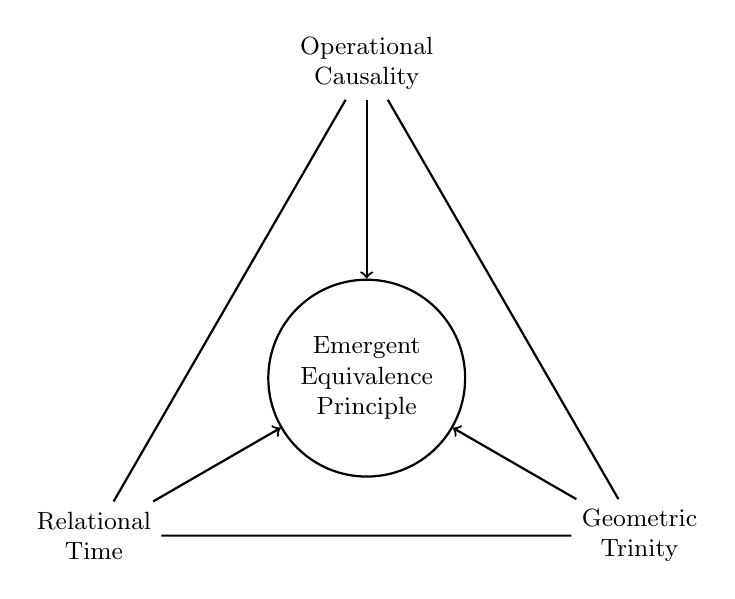
\begin{tikzpicture}[thick, every node/.style={align=center, font=\small}]
                % Triangle vertices
                \node (Causality) at (90:4) {Operational\\Causality};
                \node (RelationalTime) at (210:4) {Relational\\Time};
                \node (Trinity) at (330:4) {Geometric\\Trinity};

                % Triangle edges
                \draw[-] (Causality) -- (RelationalTime) -- (Trinity) -- (Causality);

                % Arrows from each side to center
                \node[draw, circle, minimum size=2.5cm, inner sep=2pt] (Center) at (0,0) {Emergent\\Equivalence\\Principle};

                \draw[->, thick] (Causality) -- (Center);
                \draw[->, thick] (RelationalTime) -- (Center);
                \draw[->, thick] (Trinity) -- (Center);
            \end{tikzpicture}
            \caption{Three structural ingredients yielding the Equivalence Principle as an emergent low-energy symmetry.}
            \label{fig:triad}
        \end{figure}

% ============================================================
    \section{The Equivalence Principle Reconsidered}\label{sec:ep}

    \subsection{EP variants and evidence}\label{subsec:variants}
        Distinguish weak equivalence (universality of free fall), Einstein equivalence (local Lorentz and position invariance), and strong equivalence (including gravitational self-energy). Precision tests impose tight bounds in many regimes \cite{Will2014}.

    \subsection{EP as axiom in curvature-based gravity}\label{subsec:axiom}
        In standard GR pedagogy, the EP motivates locally inertial frames that remove gravitational effects by coordinates, suggesting gravity is geometry rather than force. Powerful—but not unique—especially in metric--affine or gauge formulations \cite{ManciniTinoCapozziello2025}.

    \subsection{EP as emergent in teleparallel and symmetric teleparallel}\label{subsec:teleparallel}
        TEGR and STEGR separate inertial and gravitational contributions at the level of the connection, allowing EP-like phenomenology without taking the EP as fundamental. This supports an emergent reading tied to connection dynamics \cite{ManciniTinoCapozziello2025,BeltranJimenez2018,AldrovandiPereira2013}.

        \begin{remark}[Didactic recap]
            \emph{Quick map.} WEP: motion $\sim$ mass-independence; EEP: local nongravitational physics respects SR; SEP: even gravitational self-energy obeys equivalence. The present account preserves the tested content while shifting the interpretive load from axiom to emergence.
        \end{remark}

% ============================================================
    \section{Emergence of the EP from Relational Time and Connection Dynamics}\label{sec:emergence}

    \subsection{Synthesis}\label{subsec:synthesis}
        Combine: (i) causality fixes the Lorentzian scaffold \cite{Pineda2026,Zeeman1964}; (ii) relational constraints yield redshift and energy--energy interactions at low energy \cite{SinghFriedrich2025,PageWootters1983}; and (iii) geometric codings are empirically equivalent \cite{ManciniTinoCapozziello2025,BeltranJimenez2018}. In this regime, the EP is an emergent organizing principle.

    \subsection{Low-energy universality}\label{subsec:universality}
        The effective coupling depends on energy operators rather than composition-specific constants. Universality of free fall and equality of inertial and gravitational mass then appear as consequences of the relational structure, not separate postulates \cite{SinghFriedrich2025,ManciniTinoCapozziello2025}.

    \subsection{When deviations should appear}\label{subsec:deviations}
        Deviations should track clock resolution, energy superpositions in the source, or departures from the perturbative regime. These deviations are coherence-dependent corrections to conditional evolution, not classical fifth forces, and they scale as $\epsilonL^2$ for systems approaching the perturbative boundary. Observable signatures include phase decoherence between non-identical quantum clocks and redshift modulations correlated with internal energy superpositions \cite{SmithAhmadi2020,CastroRuiz2017}.

        \begin{remark}[Didactic recap]
            \emph{One-sentence logic.} Causality $\Rightarrow$ Lorentz scaffold; relational time $+$ small deformation $\Rightarrow$ redshift \& energy–energy term; geometric trinity $\Rightarrow$ multiple codings; together $\Rightarrow$ EP as a low-energy symmetry with clear conditions for small deviations.
        \end{remark}

        The overall logical flow is depicted in Fig.~\ref{fig:flowchart}.

        \begin{figure}[ht]
            \centering
            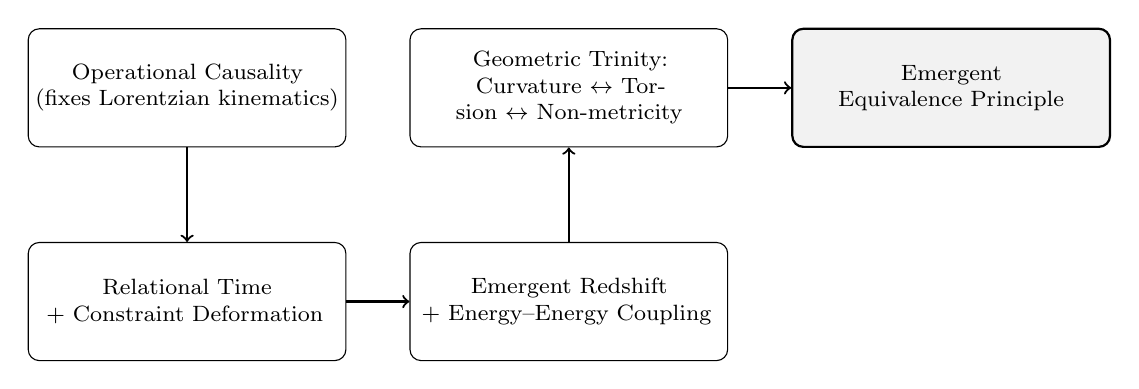
\begin{tikzpicture}[
                every node/.style={draw, rectangle, rounded corners=4pt, align=center, font=\footnotesize, text width=3.8cm, minimum height=1.5cm},
                arrow/.style={->, thick}
            ]

% Top row
                \node (Causality) {Operational Causality\\(fixes Lorentzian kinematics)};
                \node[below=1.2cm of Causality] (RelTime) {Relational Time\\+ Constraint Deformation};
                \node[right=0.8cm of Causality] (Trinity) {Geometric Trinity:\\Curvature $\leftrightarrow$ Torsion $\leftrightarrow$ Non-metricity};
                \node[below=1.2cm of Trinity] (EffHam) {Emergent Redshift\\+ Energy--Energy Coupling};

% Bottom row
                \node[right=0.8cm of Trinity, draw, thick, fill=gray!10] (EP) {Emergent\\Equivalence Principle};

% Arrows (top row)
                \draw[arrow] (Causality) -- (RelTime);
                \draw[arrow] (RelTime) -- (EffHam);

% Arrow down
                \draw[arrow] (EffHam) -- (Trinity);

% Bottom row arrows
                \draw[arrow] (Trinity) -- (EP);

            \end{tikzpicture}
            \caption{Logical flow from causal and relational structure to the emergence of the Equivalence Principle, shown as a two-row horizontal layout.}
            \label{fig:flowchart}
        \end{figure}


% ============================================================
    \section{Phenomenology and Outlook}\label{sec:phenom}

    \subsection{Consistency with weak-field tests}\label{subsec:consistency}
        Standard redshift and Newtonian limits are recovered once $\Lambda^{-1}$ is matched to the Newtonian potential scale \cite{SinghFriedrich2025,Will2014}. The geometric trinity ensures equivalent classical phenomenology across codings \cite{ManciniTinoCapozziello2025,BeltranJimenez2018}.

    \subsection{Quantum-clock probes}\label{subsec:qclocks}
        Quantum-clock interferometry and related setups directly target coherence-dependent redshift corrections and offer clean tests of the relational mechanism \cite{SmithAhmadi2020,CastroRuiz2017}. In particular, experiments comparing atomic or optical lattice clocks at different gravitational potentials could detect the predicted coherence-dependent phase lags once the relative clock energy scales approach $\\epsilonL \sim 10^{-3}$. These effects would manifest as slight deviations from standard gravitational redshift that depend on clock-state superpositions rather than composition or mass. Modern quantum-clock interferometers already reach sensitivities where $\\epsilonL \sim 10^{-3}$ is plausible. Comparing optical-lattice clocks at different potentials could reveal coherence-dependent phase lags as slight deviations from standard gravitational redshift---effects controlled by the ratio $\\epsilonL = \lVert \hat{H}_S\rVert/\Lambda$.

    \subsection{Open problem: distance}\label{subsec:openproblem}
        A principled derivation of the $1/r$ form remains. Operational distance compatible with causal structure exists \cite{Pineda2026}; importing it into the relational constraint is a concrete next step.

        \begin{remark}[Didactic recap]
            \emph{For the experimental reader.} What’s fixed now: leading redshift and Newtonian limits. What’s to measure: coherence-dependent corrections. What’s missing theoretically: an intrinsic route to $1/r$ from spatial reference frames within the same relational scaffold.
        \end{remark}

% ============================================================
    \section{Discussion}\label{sec:discussion}
    The account offered here keeps phenomenology intact while reordering foundations: causality sets the inertial scaffold; relational time and mild constraint deformations supply effective gravitational structure; and different geometric codings summarize the same empirical content. On this reading, the EP is a low-energy symmetry. The framework highlights coherence-dependent redshift as an actionable experimental target.

    Looking ahead, quantum-clock interferometry and relativistic coherence tests provide the clearest path to probing the emergent regime described here. The present account thus positions the Equivalence Principle not merely as a cornerstone of geometry but as an experimentally accessible low-energy symmetry arising from relational dynamics amenable to falsification as clock coherence and energy resolution improve.
% ============================================================
    \section{Conclusion}\label{sec:conclusion}
    Operational causality fixes relativistic kinematics \cite{Pineda2026,Zeeman1964}. Relational-time dynamics with weak deformations generate redshift and energy--energy interactions \cite{SinghFriedrich2025,PageWootters1983}. The geometric trinity reveals multiple, inequivalent geometric summaries of identical phenomenology \cite{ManciniTinoCapozziello2025,BeltranJimenez2018}. Together these motivate treating the EP as emergent and identify quantum-clock tests as the right place to look for coherence-dependent corrections.

% ============================================================
    \backmatter

    \bmhead{Acknowledgements}
    Not applicable.

    \bmhead{Declarations}

    \subsection*{Funding}
        Not applicable.

    \subsection*{Competing interests}
        The author declares no competing interests.

    \subsection*{Ethics approval}
        Not applicable.

    \subsection*{Consent to participate}
        Not applicable.

    \subsection*{Consent for publication}
        Not applicable.

    \subsection*{Data availability}
        Not applicable.

    \subsection*{Code availability}
        Not applicable.

    \subsection*{Author contributions}
        O.I. conceived the study, developed the analysis, performed the derivations, and wrote the manuscript.

% ============================================================
        \appendix
    \section{Operator Domains and Regularization of Effective Evolution}\label{app:domains}
    The expression $\hat{H}_{\rm eff}=\hat{H}_S(\hat{I}+\hat{H}_S/\Lambda)^{-1}$ requires care when $\hat{H}_S$ is unbounded or when the spectrum overlaps $-\Lambda$. In practice one can: (i) restrict to low-energy sectors $|\hat{H}_S|\ll \Lambda$ and use the expansion \eqref{eq:Heff_expand}; (ii) model clocks/systems with bounded spectra; or (iii) introduce spectral cutoffs or smearing representing finite clock resolution. These standard choices make the relational evolution well-defined \cite{SinghFriedrich2025,PageWootters1983}.

% ============================================================
% References
% ============================================================
    \begin{thebibliography}{99}

        \bibitem{Pineda2026}
        A.~Pineda,
        \textit{Relativity: A Matter of Causality},
        Foundations of Physics \textbf{56} (2026) 2.
        doi:10.1007/s10701-025-00897-4

        \bibitem{Zeeman1964}
        E.~C.~Zeeman,
        \textit{Causality implies the Lorentz group},
        Journal of Mathematical Physics \textbf{5} (1964) 490--493.
        doi:10.1063/1.1704140

        \bibitem{Kreinovich1994}
        V.~Kreinovich,
        \textit{Approximately measured causality implies the Lorentz group: Alexandrov--Zeeman result made more realistic},
        International Journal of Theoretical Physics \textbf{33} (1994) 1733--1747.
        doi:10.1007/BF00672697

        \bibitem{PageWootters1983}
        D.~N.~Page and W.~K.~Wootters,
        \textit{Evolution without evolution: Dynamics described by stationary observables},
        Physical Review D \textbf{27} (1983) 2885.
        doi:10.1103/PhysRevD.27.2885

        \bibitem{Wootters1984}
        W.~K.~Wootters,
        \textit{``Time'' replaced by quantum correlations},
        International Journal of Theoretical Physics \textbf{23} (1984) 701--711.
        doi:10.1007/BF02214098

        \bibitem{DeWitt1967}
        B.~S.~DeWitt,
        \textit{Quantum Theory of Gravity. II. The Manifestly Covariant Theory},
        Physical Review \textbf{162} (1967) 1195--1239.
        doi:10.1103/PhysRev.162.1195

        \bibitem{ManciniTinoCapozziello2025}
        C.~Mancini, G.~M.~Tino, and S.~Capozziello,
        \textit{Equivalent Gravities and Equivalence Principle: Foundations and Experimental Implications},
        Foundations of Physics \textbf{56} (2026) 1 (online 2025).
        doi:10.1007/s10701-025-00882-x

        \bibitem{AldrovandiPereira2013}
        R.~Aldrovandi and J.~G.~Pereira,
        \textit{Teleparallel Gravity: An Introduction},
        Springer (2013).
        doi:10.1007/978-94-007-5143-9

        \bibitem{BeltranJimenez2018}
        J.~Beltr\'an~Jim\'enez, L.~Heisenberg, and T.~S.~Koivisto,
        \textit{Coincident General Relativity},
        Physical Review D \textbf{98} (2018) 044048.
        doi:10.1103/PhysRevD.98.044048

        \bibitem{Will2014}
        C.~M.~Will,
        \textit{The Confrontation between General Relativity and Experiment},
        Living Reviews in Relativity \textbf{17} (2014) 4.
        doi:10.12942/lrr-2014-4

        \bibitem{SmithAhmadi2020}
        A.~R.~H.~Smith and M.~Ahmadi,
        \textit{Quantum clocks observe classical and quantum time dilation},
        Nature Communications \textbf{11} (2020) 5360.
        doi:10.1038/s41467-020-18264-4

        \bibitem{CastroRuiz2017}
        E.~Castro-Ruiz, F.~Giacomini, and \v{C}.~Brukner,
        \textit{Entanglement of quantum clocks through gravity},
        PNAS \textbf{114} (2017) E2303--E2309.
        doi:10.1073/pnas.1616427114

        \bibitem{SinghFriedrich2025}
        A.~Singh and O.~Friedrich,
        \textit{Emergence of Gravitational Potential and Time Dilation from Non-interacting Systems Coupled to a Global Quantum Clock},
        Foundations of Physics \textbf{55} (2025) 82.
        doi:10.1007/s10701-025-00893-8

        \bibitem{KarakostasZafiris2025}
        V.~Karakostas and E.~Zafiris,
        \textit{Contemporary Perspectivism as a Framework of Scientific Inquiry in Quantum Mechanics and Beyond},
        Foundations of Physics \textbf{55} (2025) 76.
        doi:10.1007/s10701-025-00888-5

    \end{thebibliography}

\end{document}